% \part*{Jeugd}

% % % % % % % % % % % % % % % % % % % % % % % % % % % % % % % % % % % % % % % % % % % % % % % % % %
% % % % % % % % % % % % % % % % % % % % % % % % % % % % % % % % % % % % % % % % % % % % % % % % % %
% % % % % % % % % % % % % % % % % % % % % % % % % % % % % % % % % % % % % % % % % % % % % % % % % %
% % % % % % % % % % % % % % % % % % % % % % % % % % % % % % % % % % % % % % % % % % % % % % % % % %
% % % % % % % % % % % % % % % % % % % % % % % % % % % % % % % % % % % % % % % % % % % % % % % % % %
% % % % % % % % % % % % % % % % % % % % % % % % % % % % % % % % % % % % % % % % % % % % % % % % % %
% % % % % % % % % % % % % % % % % % % % % % % % % % % % % % % % % % % % % % % % % % % % % % % % % %
% % % % % % % % % % % % % % % % % % % % % % % % % % % % % % % % % % % % % % %

\chapter*{Oudkarspel}

\lettrine[lines=2, loversize=0.3, lraise=0]{\initfamily I}{k} ben op 20 februari 1928 geboren. We
zijn alle drie thuis geboren met hulp van de vroedvrouw. Bert was van 1924 en Kees van 1930. Ik zat
er tussenin.

\begin{figure}[h] 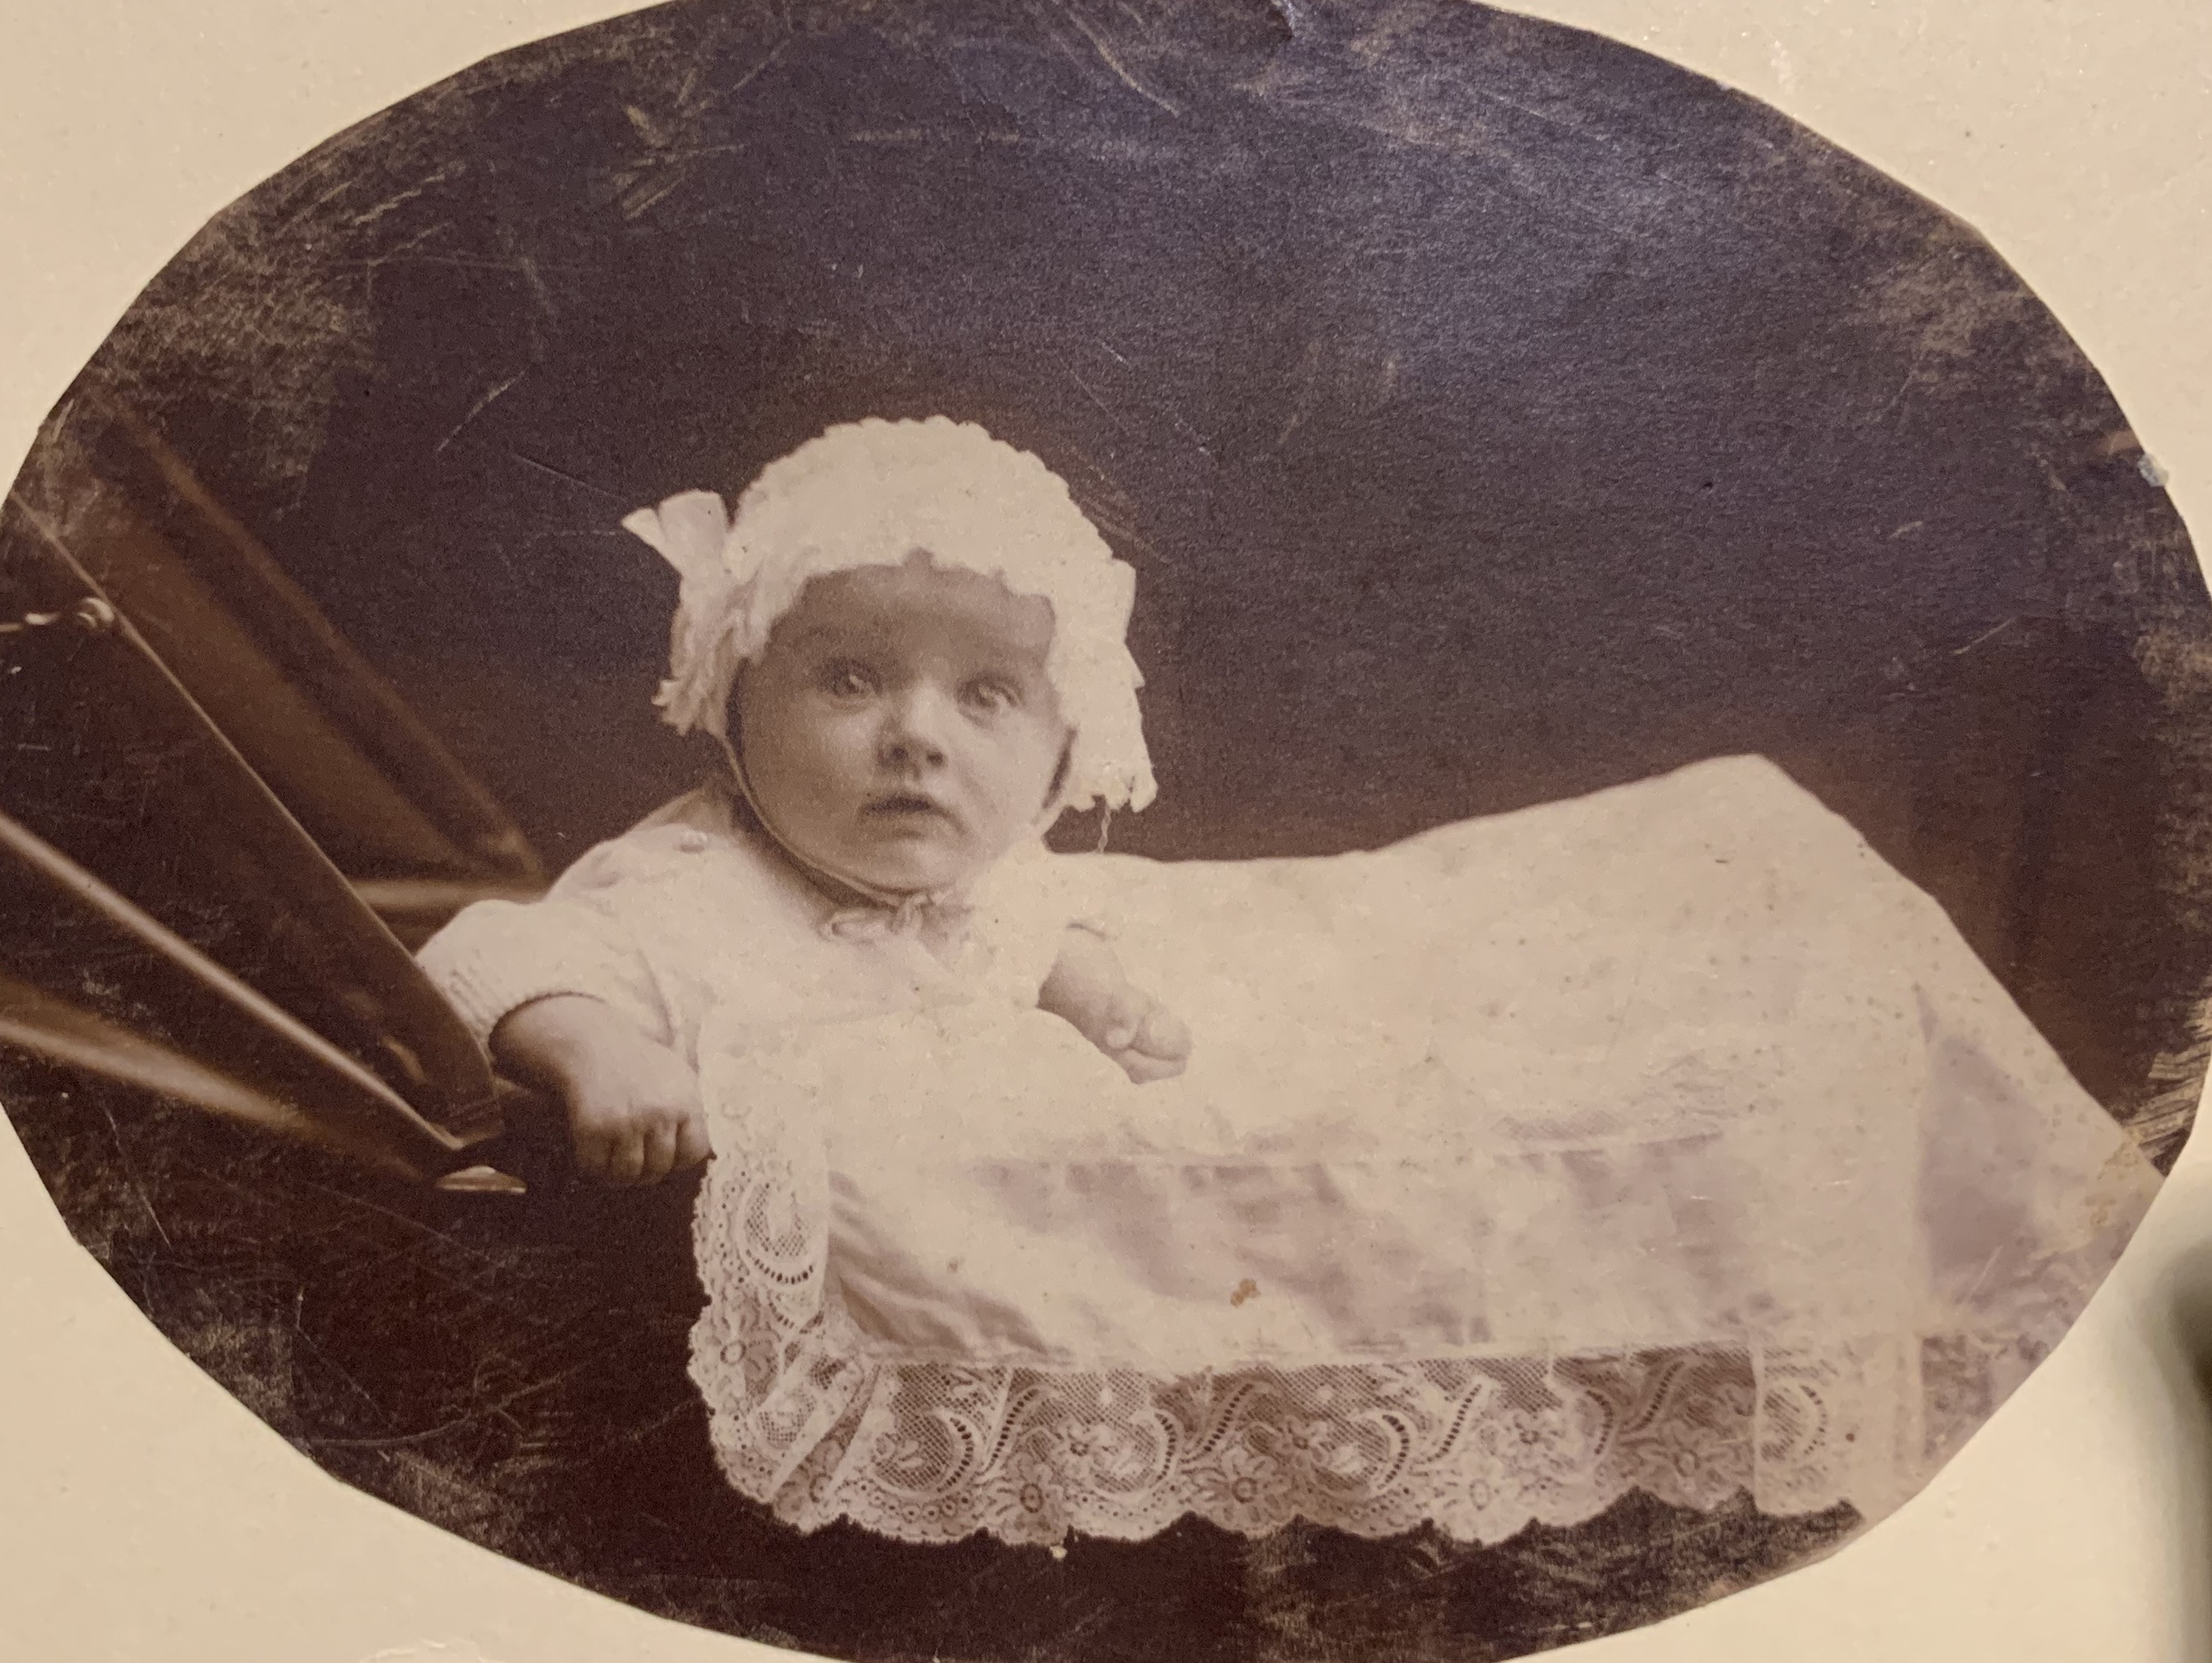
\includegraphics[width=\textwidth]{image3.jpg} \caption{Tine de Booij.}
\end{figure}

Vanaf 6 ging je lopend naar school. Het hoofd van de school woonde tegenover ons. Kwam Bert een keer
thuis met een waterpistool; ze wilden op de meester schieten maar durfden het niet. Toen vroegen ze
aan mij om dat te doen! Je weet niet hoe hard we daarna wegliepen! Toen kreeg m’n moeder de
buurman aan de deur. Ze hadden een dochter en die had een eigen speelkamer.

Ik speelde veel met Kees vroeger. We konden goed samen spelen. Kees had ook wel zijn vriendjes en ik
mijn vriendinnen. We hadden ringen in de bijkeuken hangen en een schommel buiten.

\begin{figure}[h] 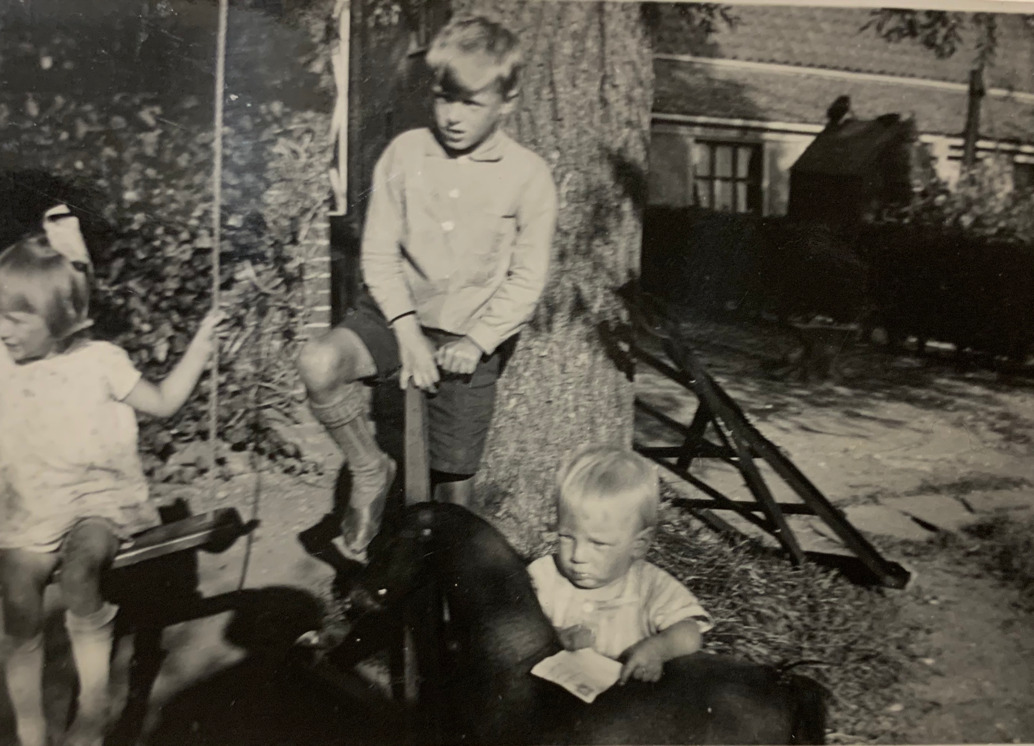
\includegraphics[width=\textwidth]{image4.jpg} \caption{De schommel in de tuin.}
\end{figure}

Mijn moeder had toen al een wasmachine; die stond in de smederij. Want daar stond een slijpmachine
en daar werd de wasmachine ook aangesloten. 

Er was een kooktoestel in de bijkeuken en in de winter zaten we daar. In het voorjaar gingen de
mooie stoelen weer naar de voorkamer en aten we daar.  \begin{figure}[h]
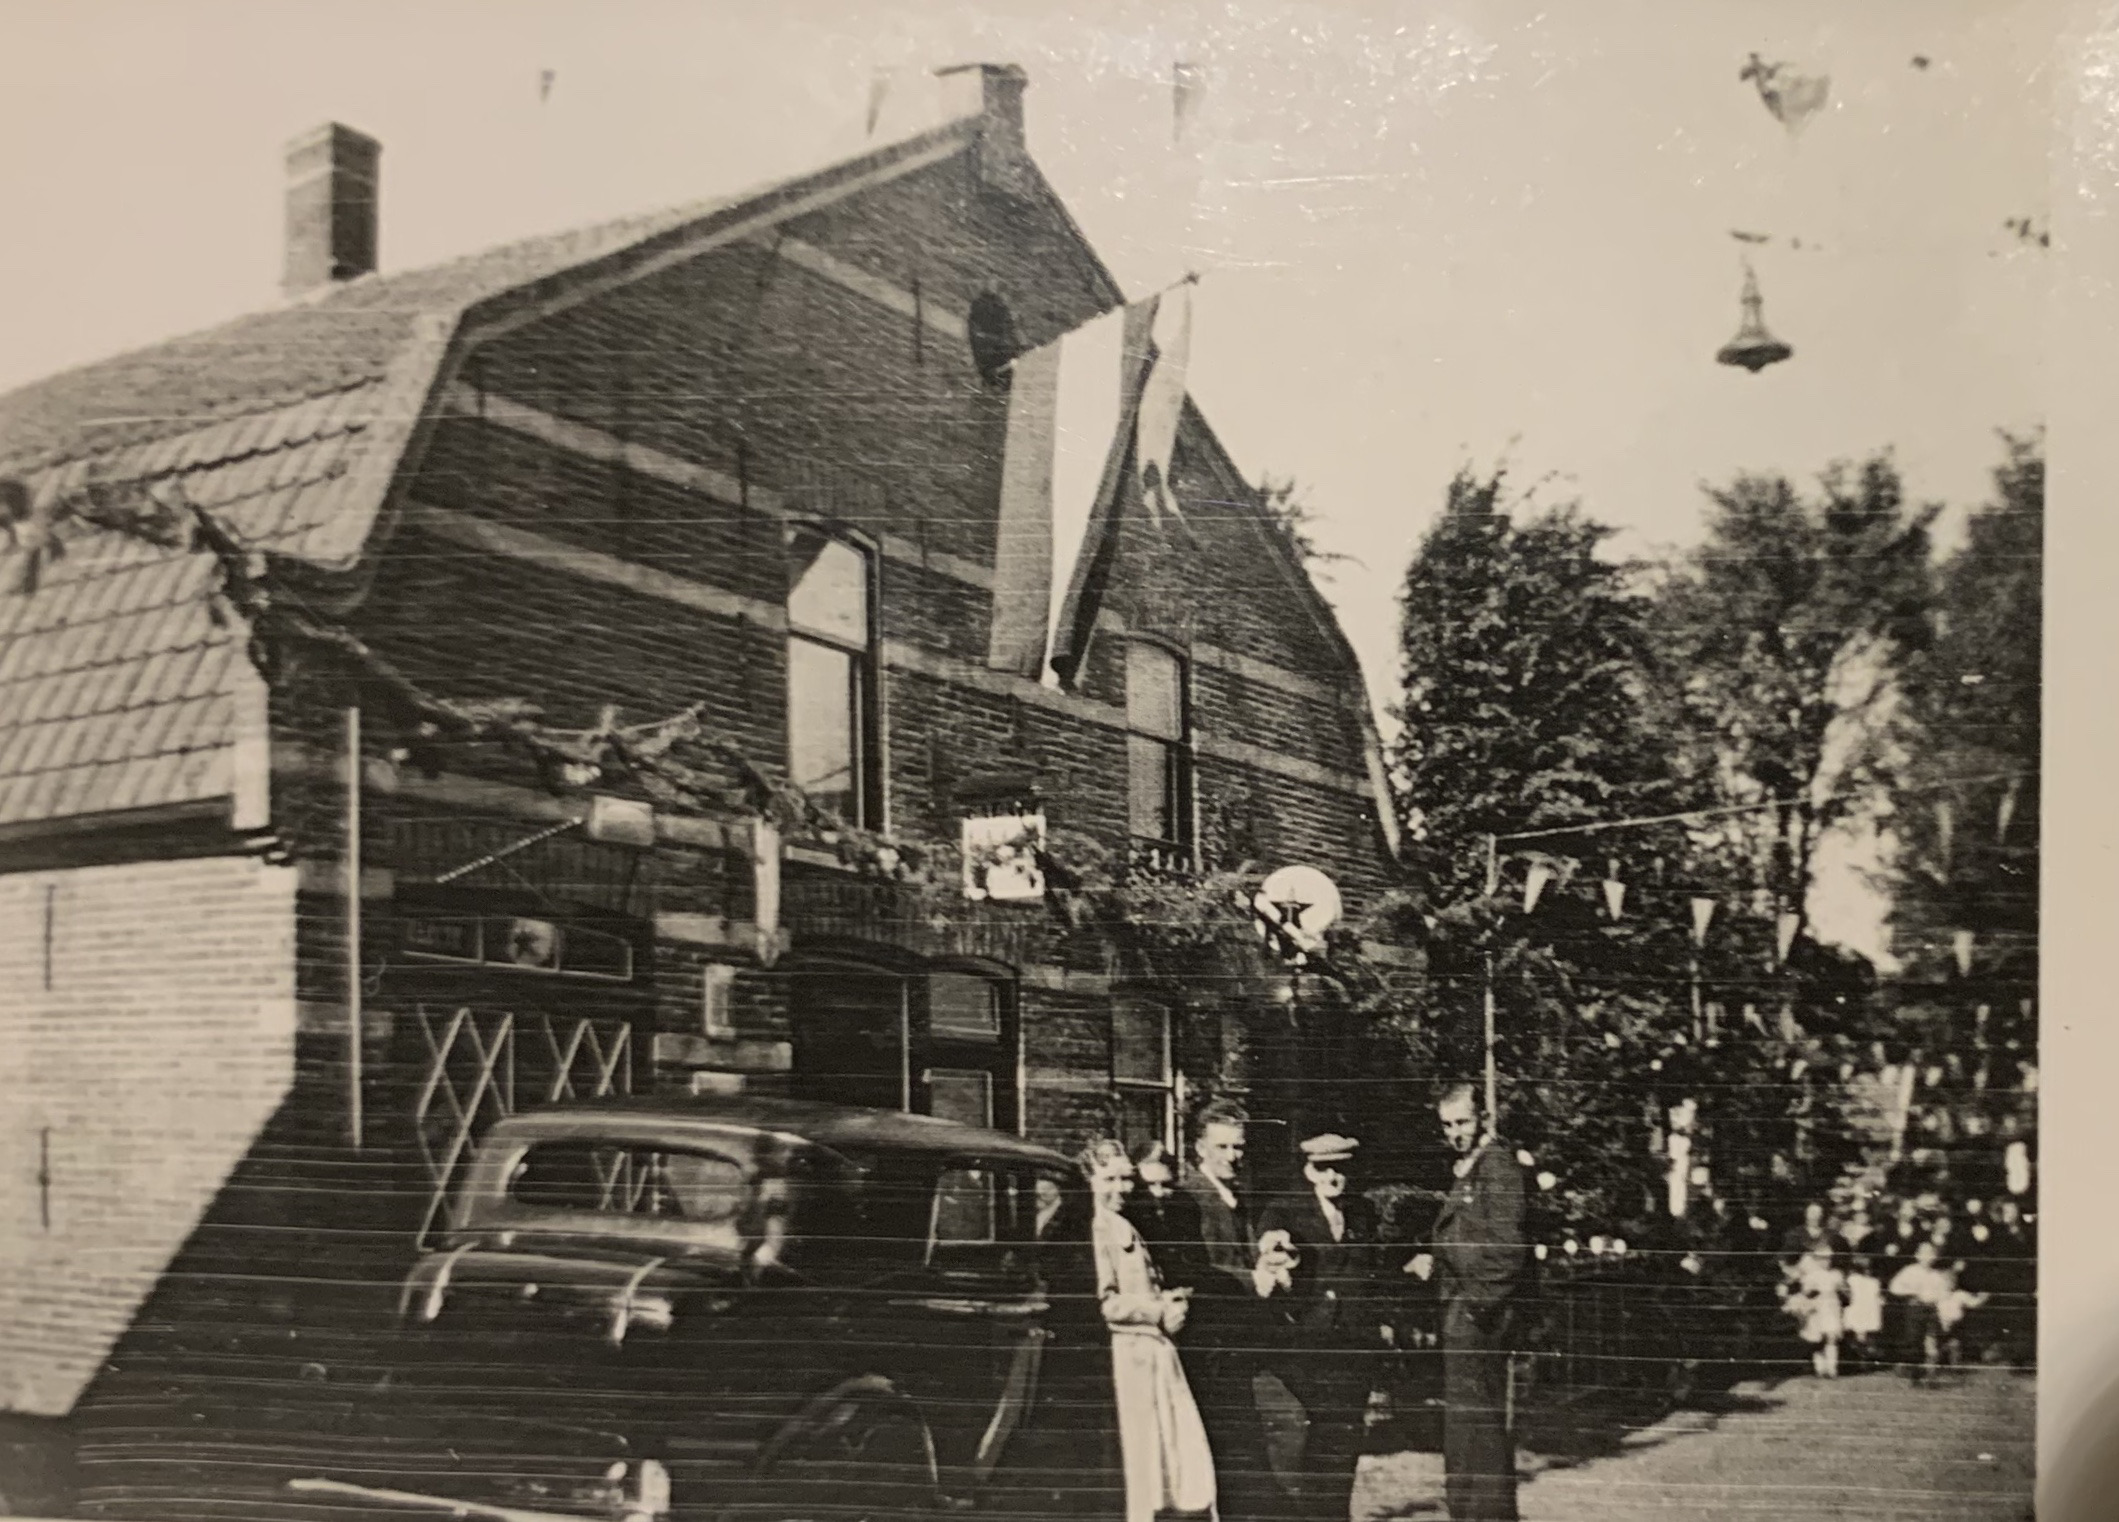
\includegraphics[width=\textwidth]{image5.jpg} \caption{Het huis in Oudkarspel} \end{figure} In de
bijkeuken was ook een bedstee en daar sliepen de jongens.  Als klein kind sliep ik in de bedstee bij
m’n ouders. Toen ik groter werd kreeg ik de kamer op zolder.  Eerst hadden we een WC buiten,
achter de garage, boven het water. Maar toen ik jong was kregen we al een WC binnen. In Langedijk,
als je daar ging varen, voer je de hele tijd onder de buiten-WC's van de mensen door.

\begin{figure}[h] 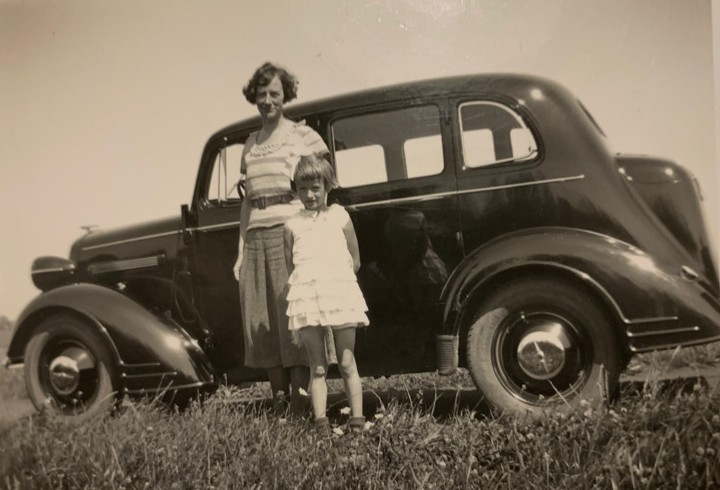
\includegraphics[width=1\textwidth]{image6.jpg} \caption{Met de auto naar het
strand.} \end{figure}

Iedere zondag gingen we naar het strand bij Camperduin. Dat was gezond vond m’n moeder.  We
hadden een grote tent mee waar je je kon verkleden. We gingen met de auto daarheen. Voor m’n
vader was dat niet altijd zo leuk want hij was dan moe van het bedrijf en het was een heel gesjouw
met al die spullen.

\begin{figure}[hp] 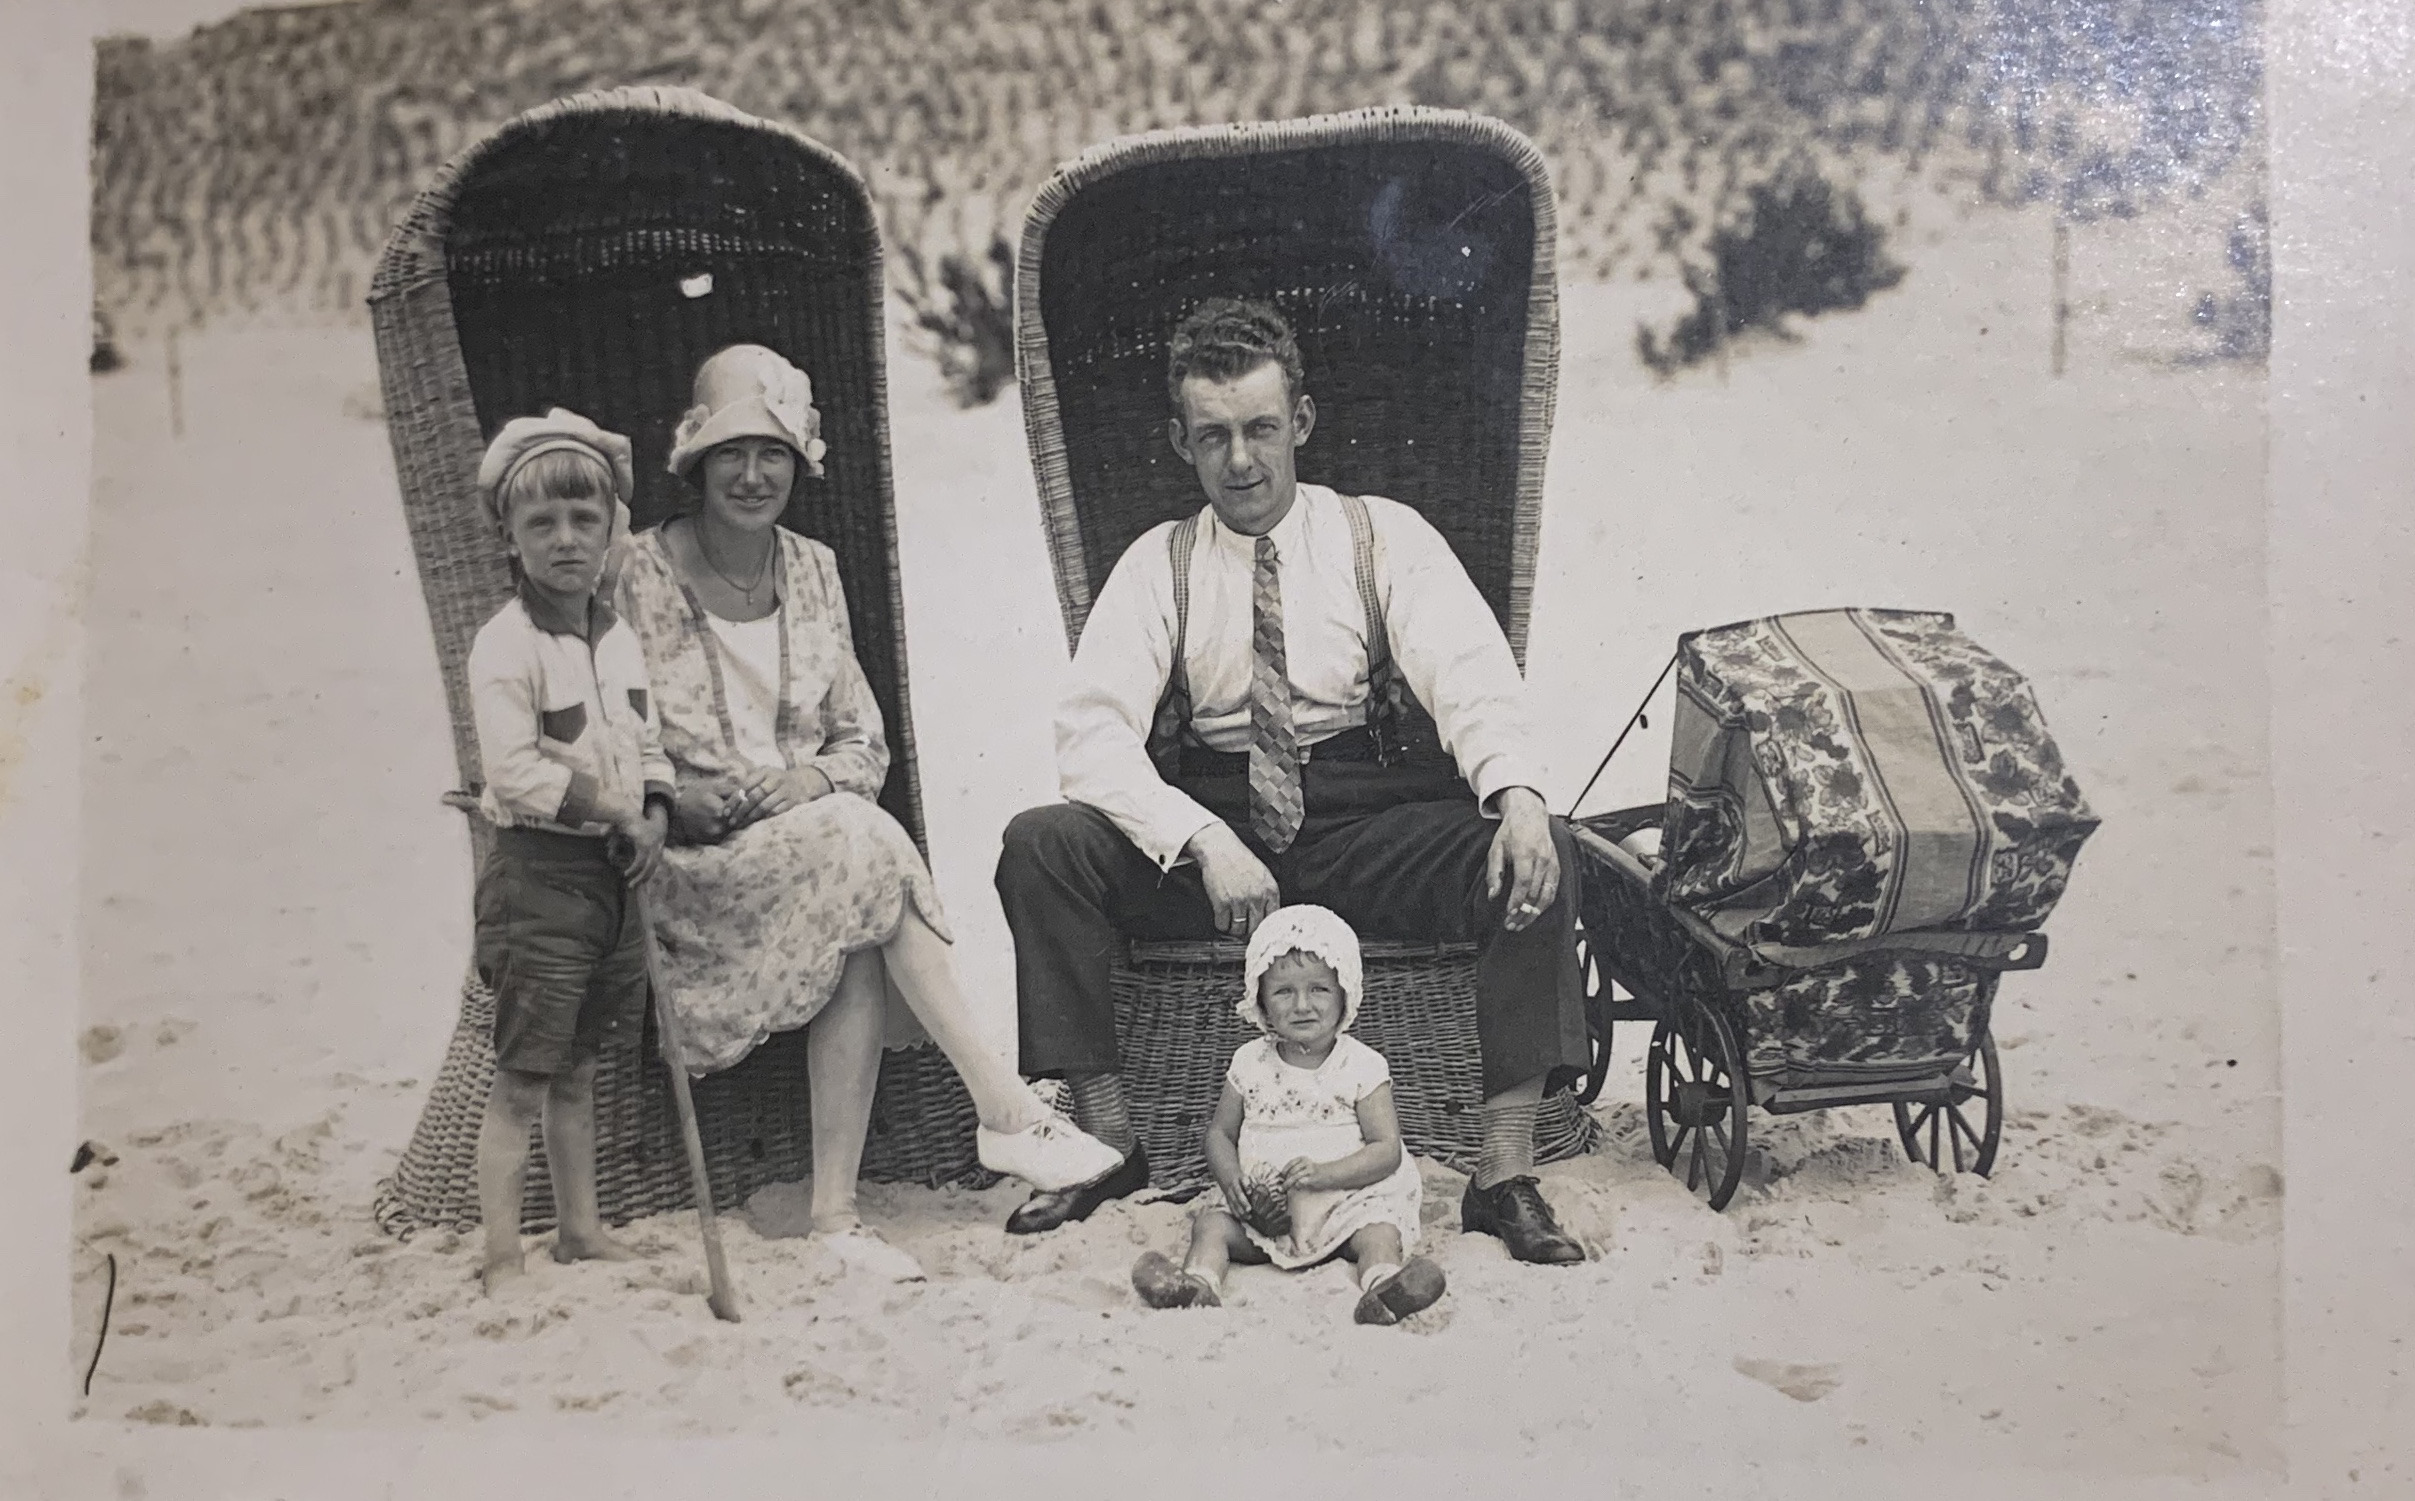
\includegraphics[width=1\textwidth]{image7.jpg} \caption{Het gezin aan het strand.}
\end{figure}

Bert was als kind altijd een beetje minnetjes. Veel ziek. Hij was heel veel op de boerderij van mijn
grootouders in Schoorldam, dan was hij gelijk buiten. 

Mijn vader heeft toen een bokkenwagen gemaakt en opa hielp om de bok voor de kar te zetten.

We gingen ook vaak nog even aan in Schoorldam, bijna elke week.

En \'{e}\'{e}n keer zijn we met opa Vlam vanaf Schoorldam met een mooi rijtuig en een paard ervoor
naar het strand geweest. Een rijtuig met van die kussens aan weerskanten. Op Camperduin kende hij
mensen waar hij het paard kon stallen. Dat was een geweldige belevenis.

\begin{figure}[h] 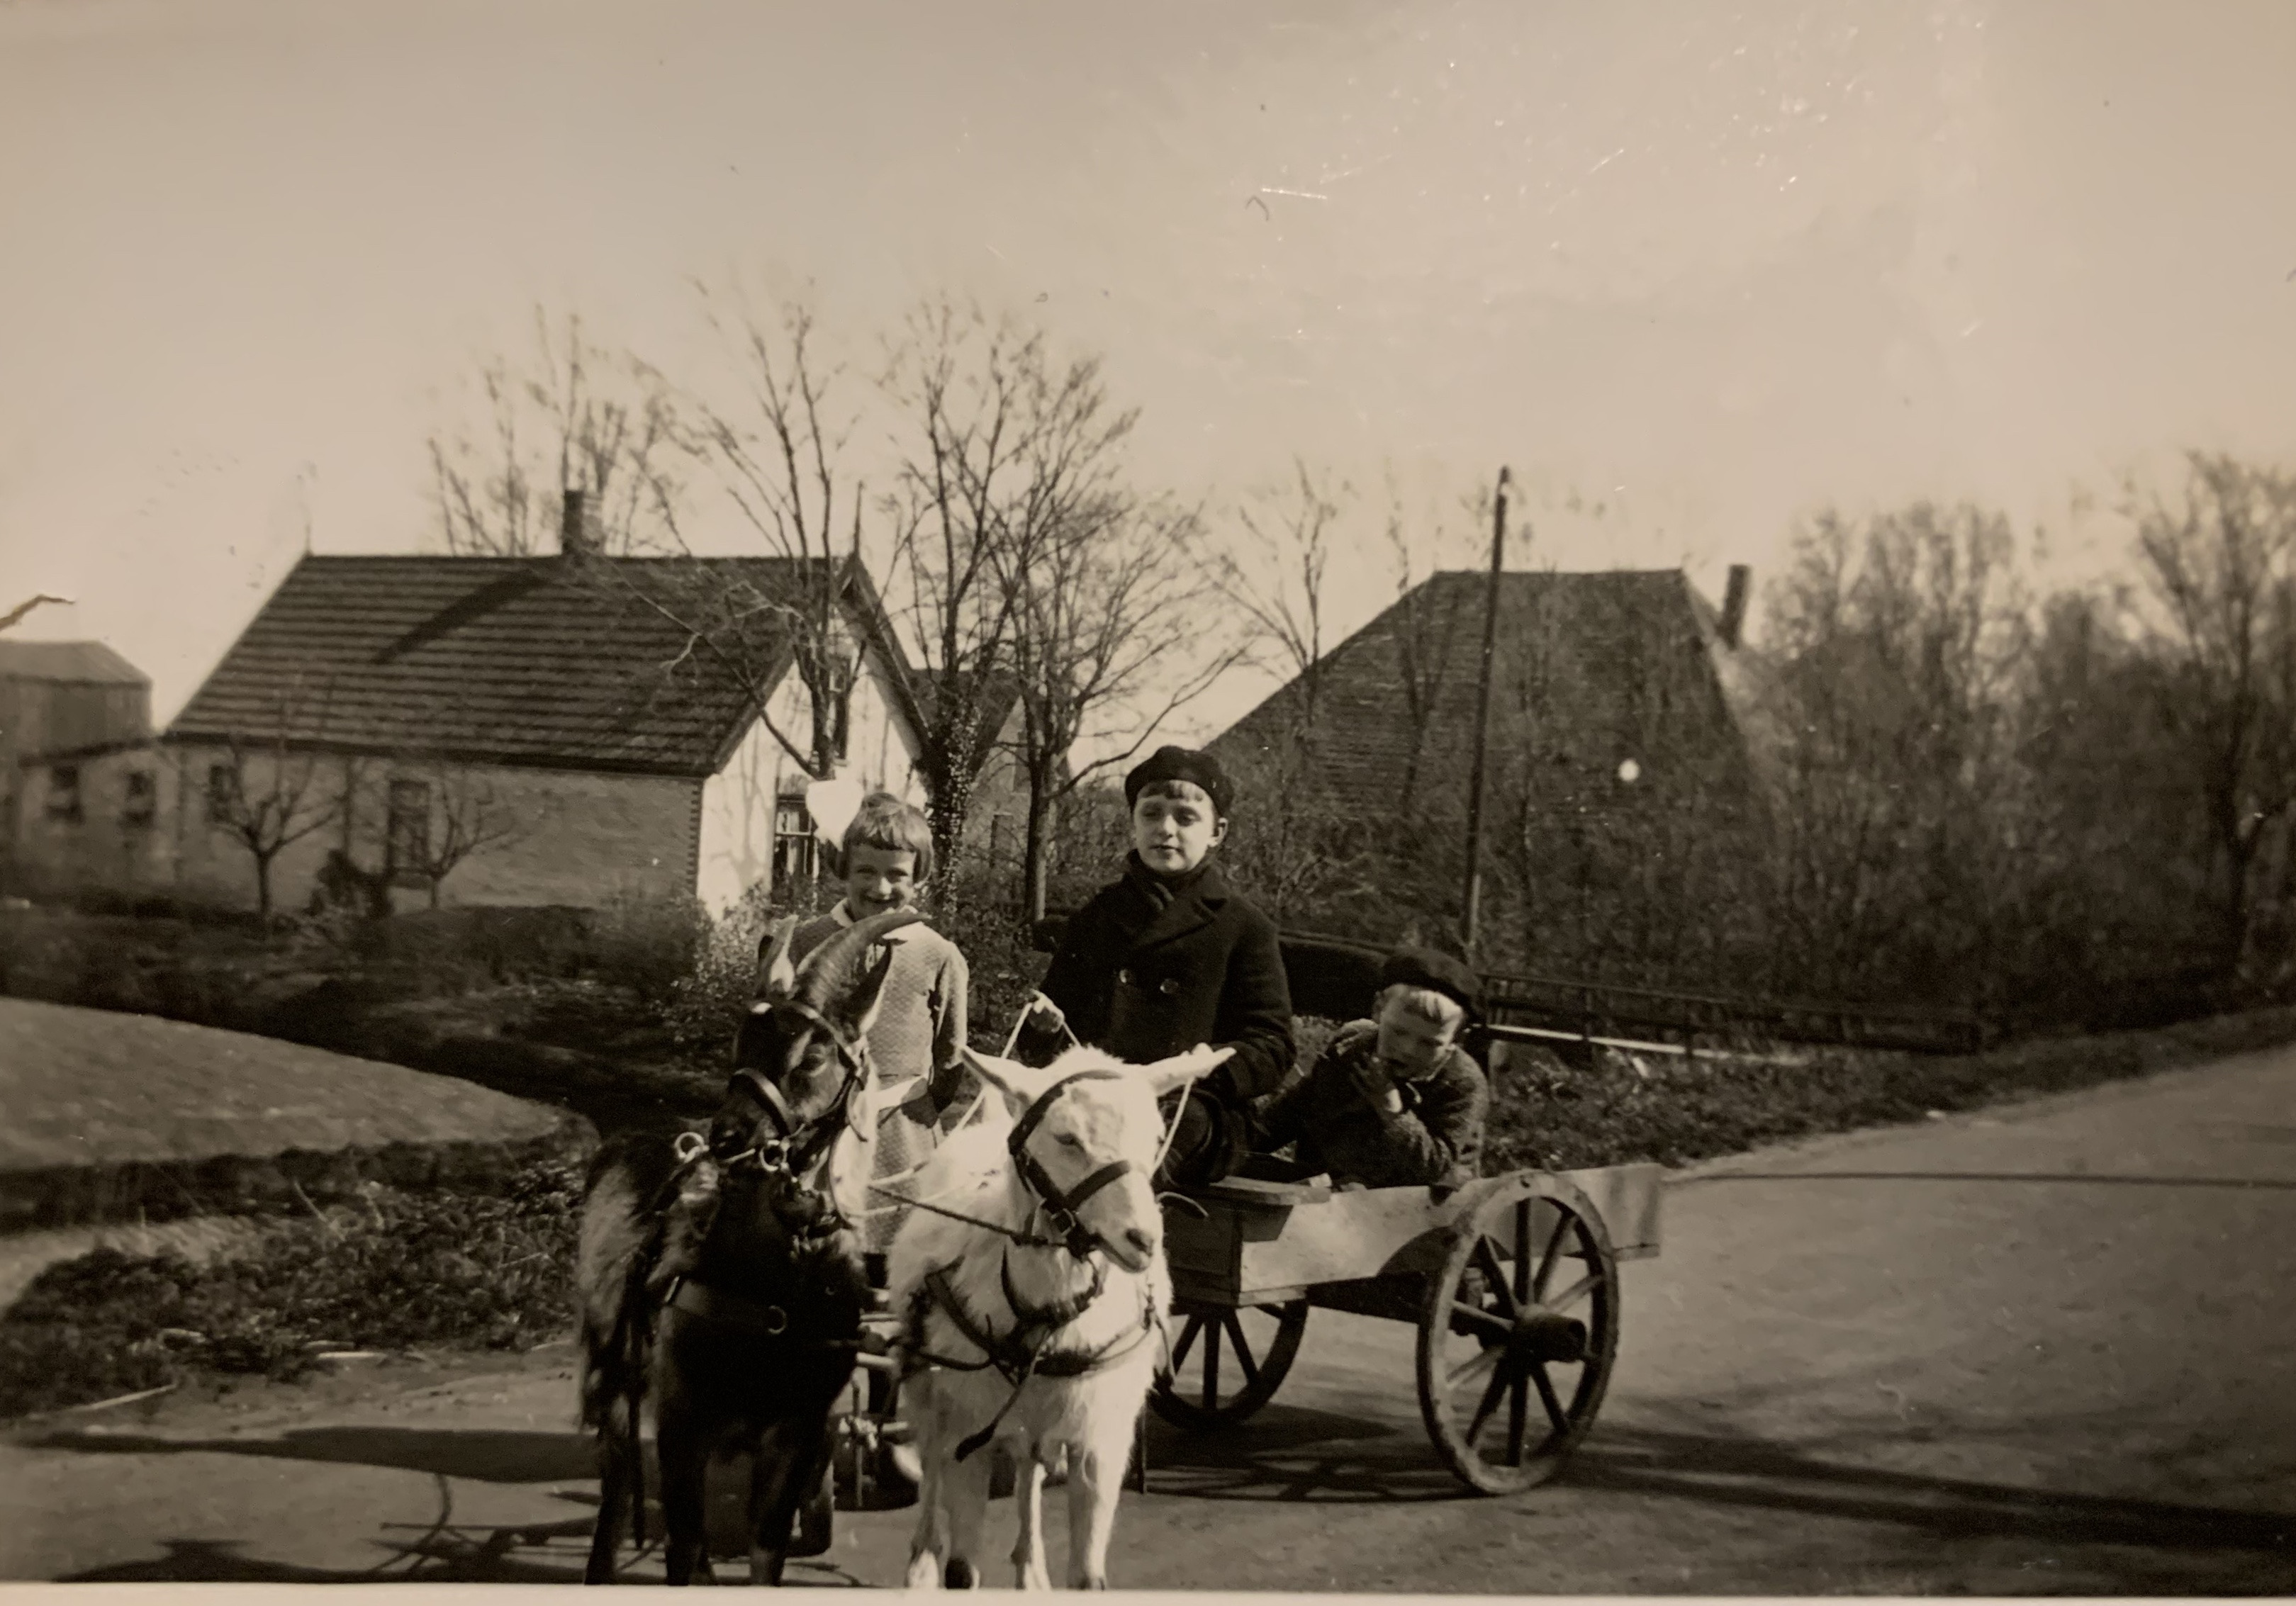
\includegraphics[width=1\textwidth]{image8.jpg} \caption{De kinderen hadden ook
een kar.} \end{figure}

Mijn vader had een heel bedrijf; een smederij, een winkel en een grote garage. Daar stond de
dorsmachine die door het hele dorp werd gehuurd. Als hij gebruikt werd stond hij op een veldje
verderop en dan kwamen alle landbouwers met hun graan; dat kwam dan in zakken. 

\begin{figure}[h] 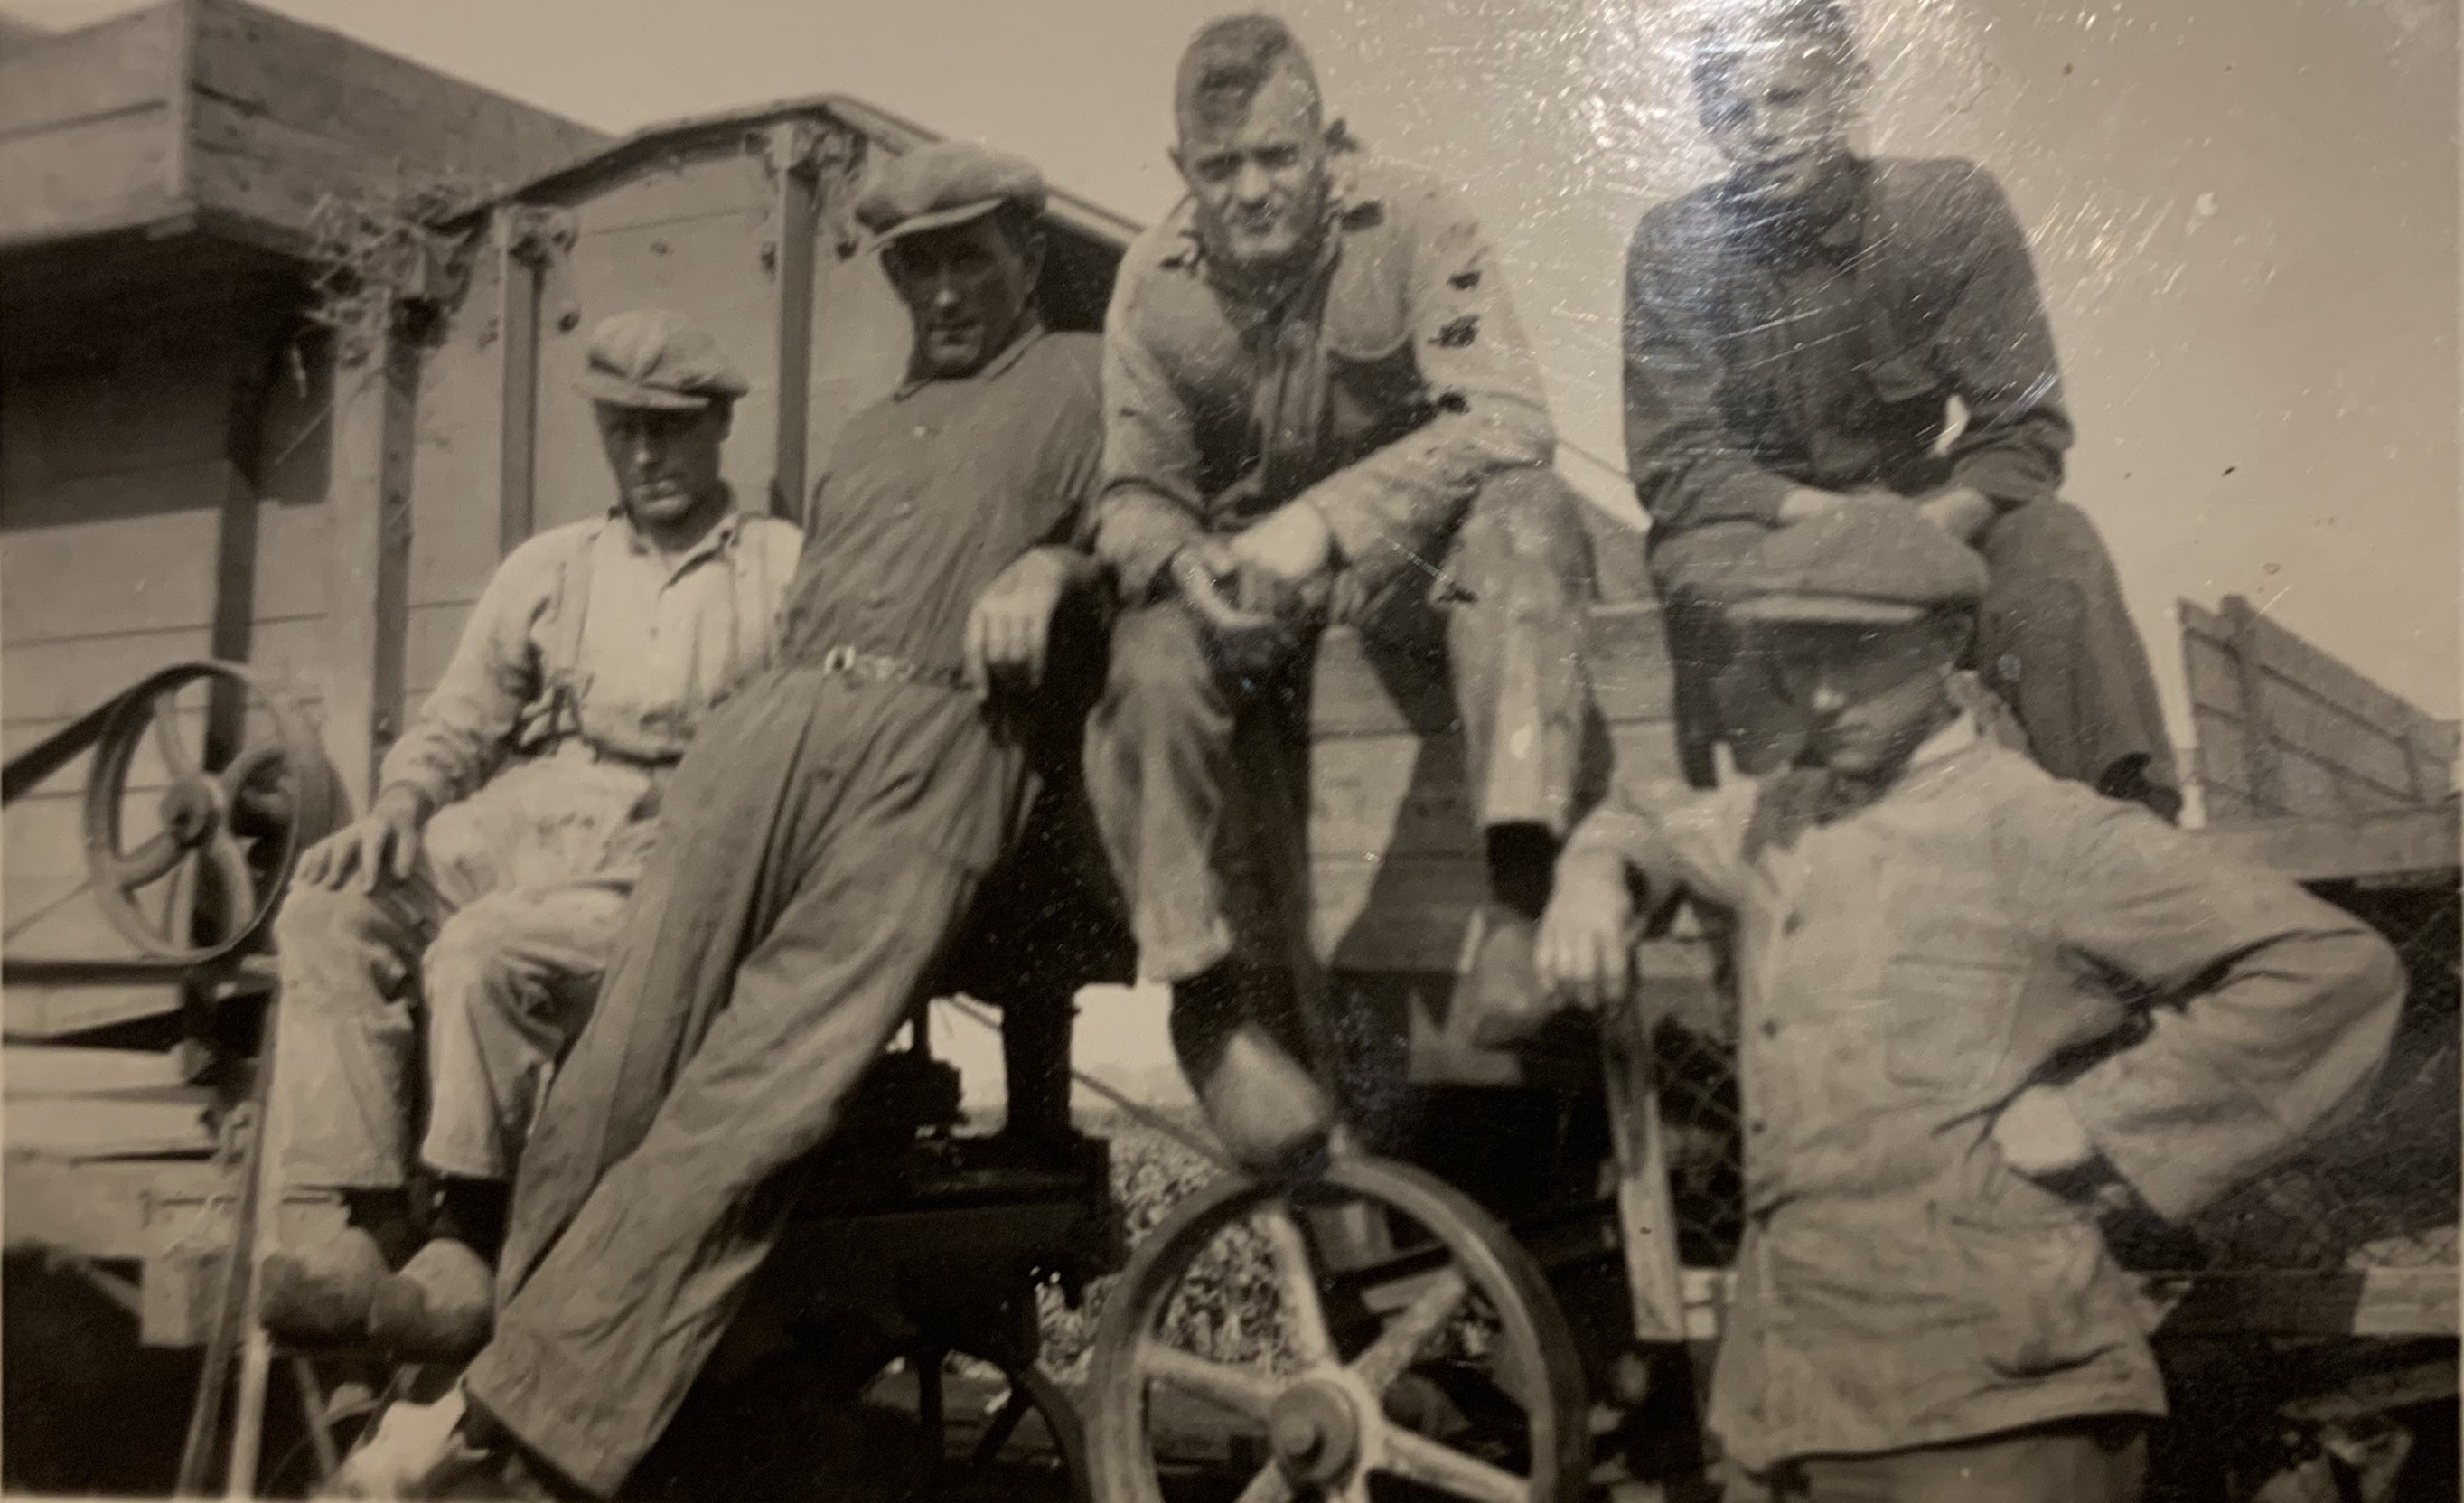
\includegraphics[width=1\textwidth]{image9.jpg} \caption{De dorsmachine.}
\end{figure}

Iedereen kwam met bootjes naar dat veld. Het land van de duizend eilanden heette het. Iedereen had
een veldje tussen het hoge water in. De bootjes werden vooruitbewogen met een kloet. Kees vond het
ook prachtig om daarbij te zijn, het dorsen.

In de garage stonden ook een aantal auto’s; die werden verhuurd.

Het huis in Oudkarpsel is later gesloopt, het staat er nu niet meer. Mijn opa en oma, de ouders van
mijn vader, woonden vlakbij. Zij woonden in een klein huisje achter ons huis. Een huisje met twee
bedsteden.

Wij roeiden ook veel. Toen ik een keer bij de dokter was zei hij dat ik zulke sterke schouders had.
Dat kwam van het roeien denk ik.

\begin{figure}[h] 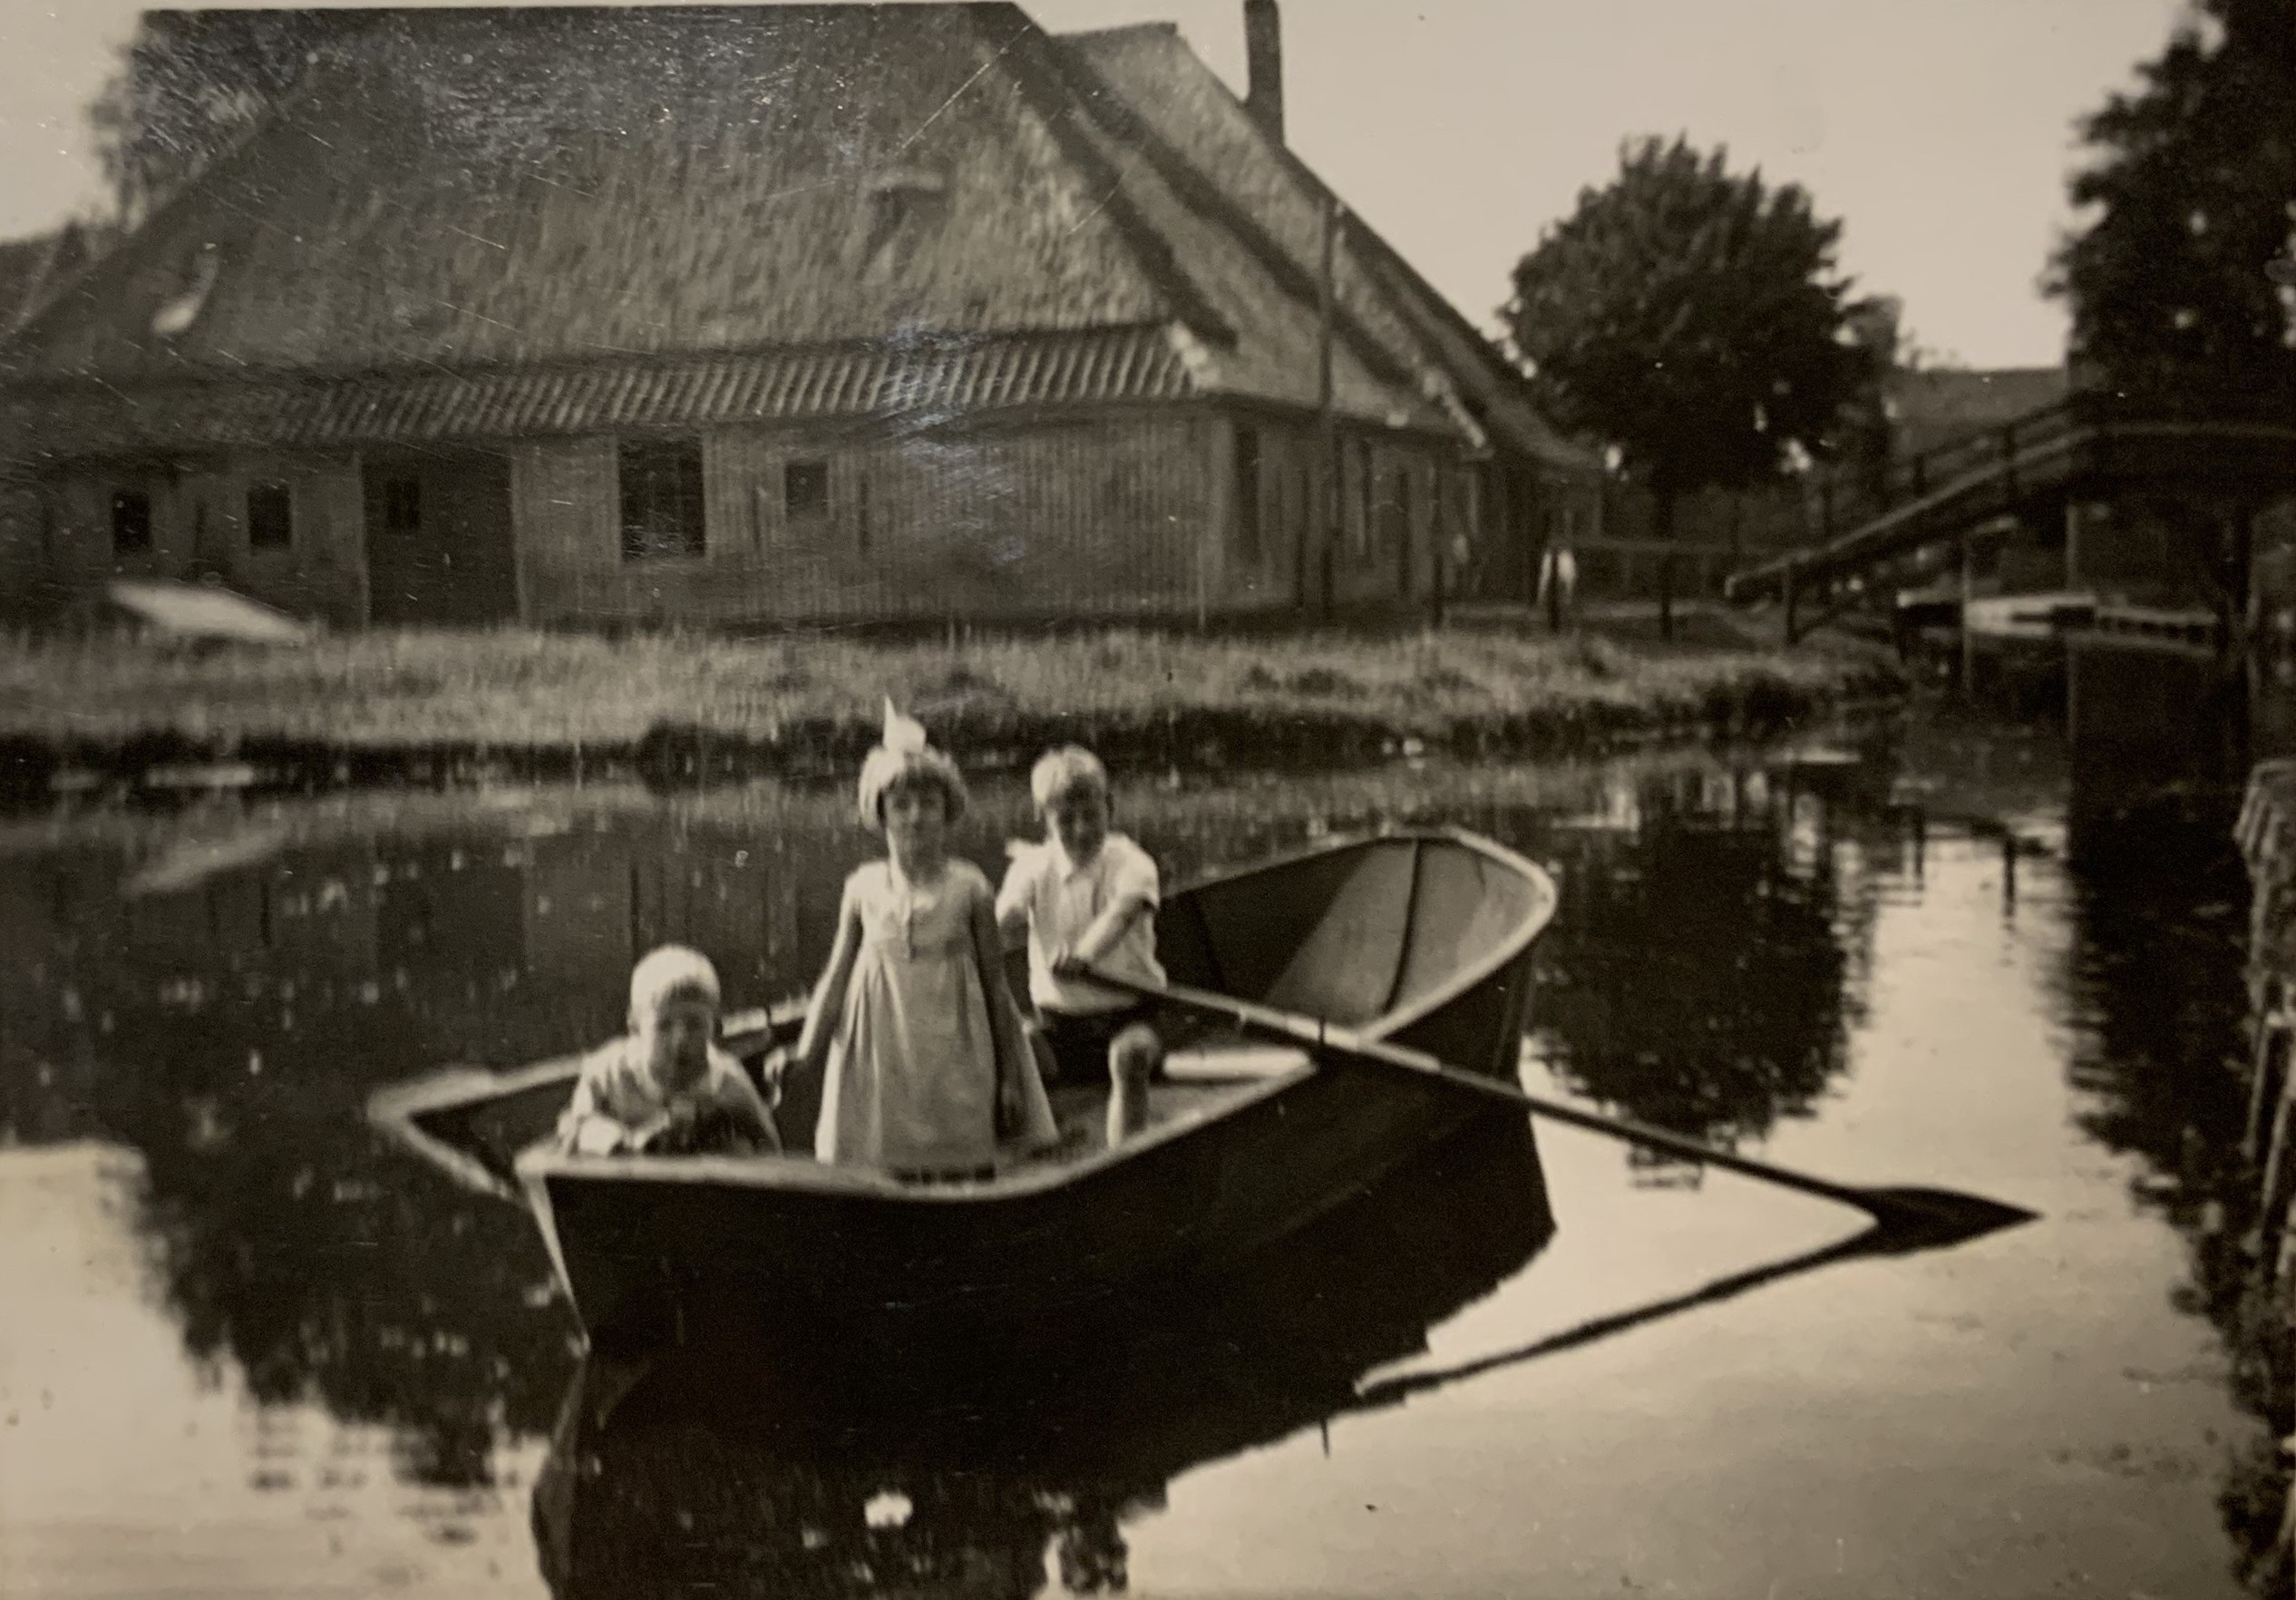
\includegraphics[width=1\textwidth]{image10.jpg} \caption{Bert aan het roeien met
Tine en Kees} \end{figure}

